\subsection{Overview}

\subsection{Interface}

\subsection{Scheduling Engine}

\subsection{System Agents}

The System Agents are used to provide the Scheduling Engine as well as the programmer (through the API) with informations about all participating systems that are relevant for scheduling descissions and job execution. \FAUST System Agents are realized as independent command line applications that run on the execution systems and report vital system and status informations like queue status, network load, etc. to back to the \FAUST instance.

\begin{figure}[bth!]
  \begin{center}
    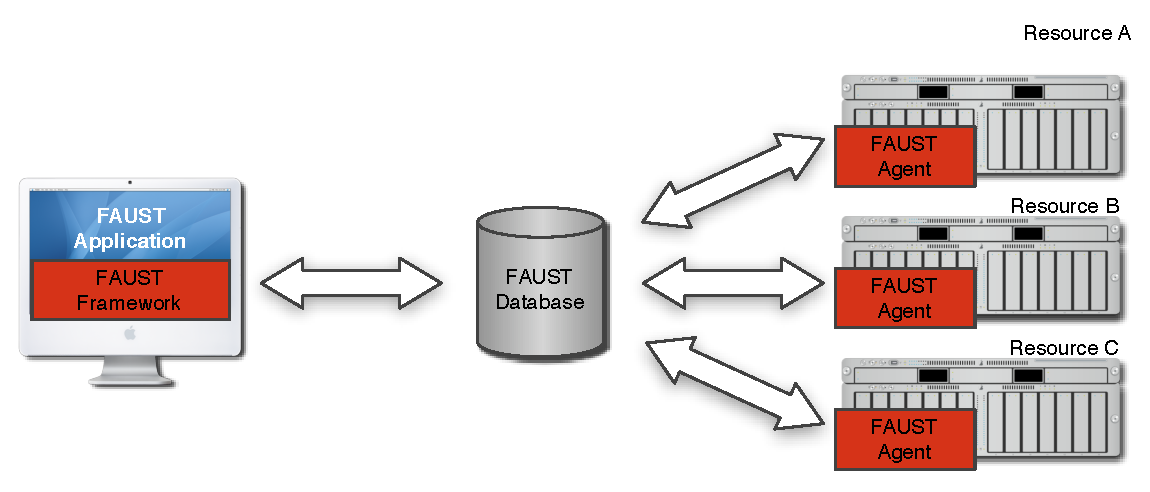
\includegraphics[width=0.95\textwidth]{figures/faust_agents_01}
    \caption{\label{fig:faust_agents_01} Example of a \FAUST application 
      instance running agents on three execution hosts. To ensure 
      application persitency, the communication between the application
      and the agents flows through a proxy database. }
  \end{center}
\end{figure}

Besides reporting system informations to the application, agents can optionally act as job submission endpoints. In this scenario, an application sends jobs directly to the agents for execution and not to the local job service (like Globus, GridSAM, PBS, etc). This will usually happen, if the application scheduler (or the programmer) decides to apply 'hijacking' strategies like \textit{Glide-In} which require circumvention of local queueing systems.

\subsubsection{Mode of Operation}

The System Agents are transparently deployed and started by a \FAUST Framework application as soon as a new \texttt{faust::service} instance gets instantiated. Each \texttt{service} instance is defined by a set of resource \texttt{descriptions} which represent targets for possible job submission. Each \texttt{resource} has its own System Agent for management, monitoring and information retreival. 

Unfortunately, different distributed infrastructures require different techniques to extract the informations that are required for effective scheduling. Although there are several more or less well defined interfaces to query these informations like \textit{NWS} or \textit{BQP}, it appears that in practice their existence and proper operation cannot be assumed. For this reason, agents require a relatively rich set of initial system informations that are used to generate subsequent runtime informations and performance predictions. Once deployed and started, System Agents loop through the following execution procedure: 


